%% ************************************************
%% Universidade Nova de Lisboa
%% NOVA Information Management School
%% Computação em Estatística e Gestão de Informação
%% Júlio Caineta, 2015
%% ************************************************
\documentclass{exam}
\usepackage[utf8]{inputenc}
\usepackage{amsmath}
\usepackage[portuguese]{babel}
\usepackage[hidelinks,pdfusetitle]{hyperref}
\author{Júlio Caineta}
\title{CEGI 2014/2015 - Exercícios 4}
\usepackage{lastpage}
\usepackage{minted}
\usepackage{gensymb}
\usepackage{wrapfig}
\usepackage{tabulary}
\usepackage{graphicx}
%\usepackage{color}
\cfoot{Página \thepage\ de \pageref{LastPage}}
\renewcommand{\solutiontitle}{\noindent\textbf{Solução:}\par\noindent}
\newminted{r}{autogobble}
\newmintinline{r}{}
 
%\printanswers
%\shadedsolutions

\begin{document}
 
\begin{center}
\textsc {\small NOVA IMS -- Universidade Nova de Lisboa} \\
\textsc {Computação em Estatística e Gestão de Informação -- 2º Semestre 2014/15}
\vspace{5mm} \\
{\large Exercícios 4}
\end{center}
 
\vspace{5mm}

\section*{Manipulação de ficheiros}

Em termos computacionais, a informação é habitualmente transmitida em blocos a que denominamos ficheiros. O \textbf{R} disponibiliza uma vasta colecção de funções para manipular ficheiros de diferentes formatos. Neste exercício, pretende-se fazer uso de algumas funções de manipulação de ficheiros, e dos objectos resultantes do seu carregamento numa sessão de \textbf{R}.

Considere o seguinte contexto. Tornou-se num reconhecido \textit{data analyst}, e uma das maiores empresas da indústria petrolífera está a requisitar os seus serviços. Eles estão a começar a explorar um novo reservatório, tendo já disponível os dados obtidos no primeiro furo (exemplo ilustrativo na \autoref{fig:pump}).

\begin{figure}[h]
	%\vspace{-40pt}
	\centering
	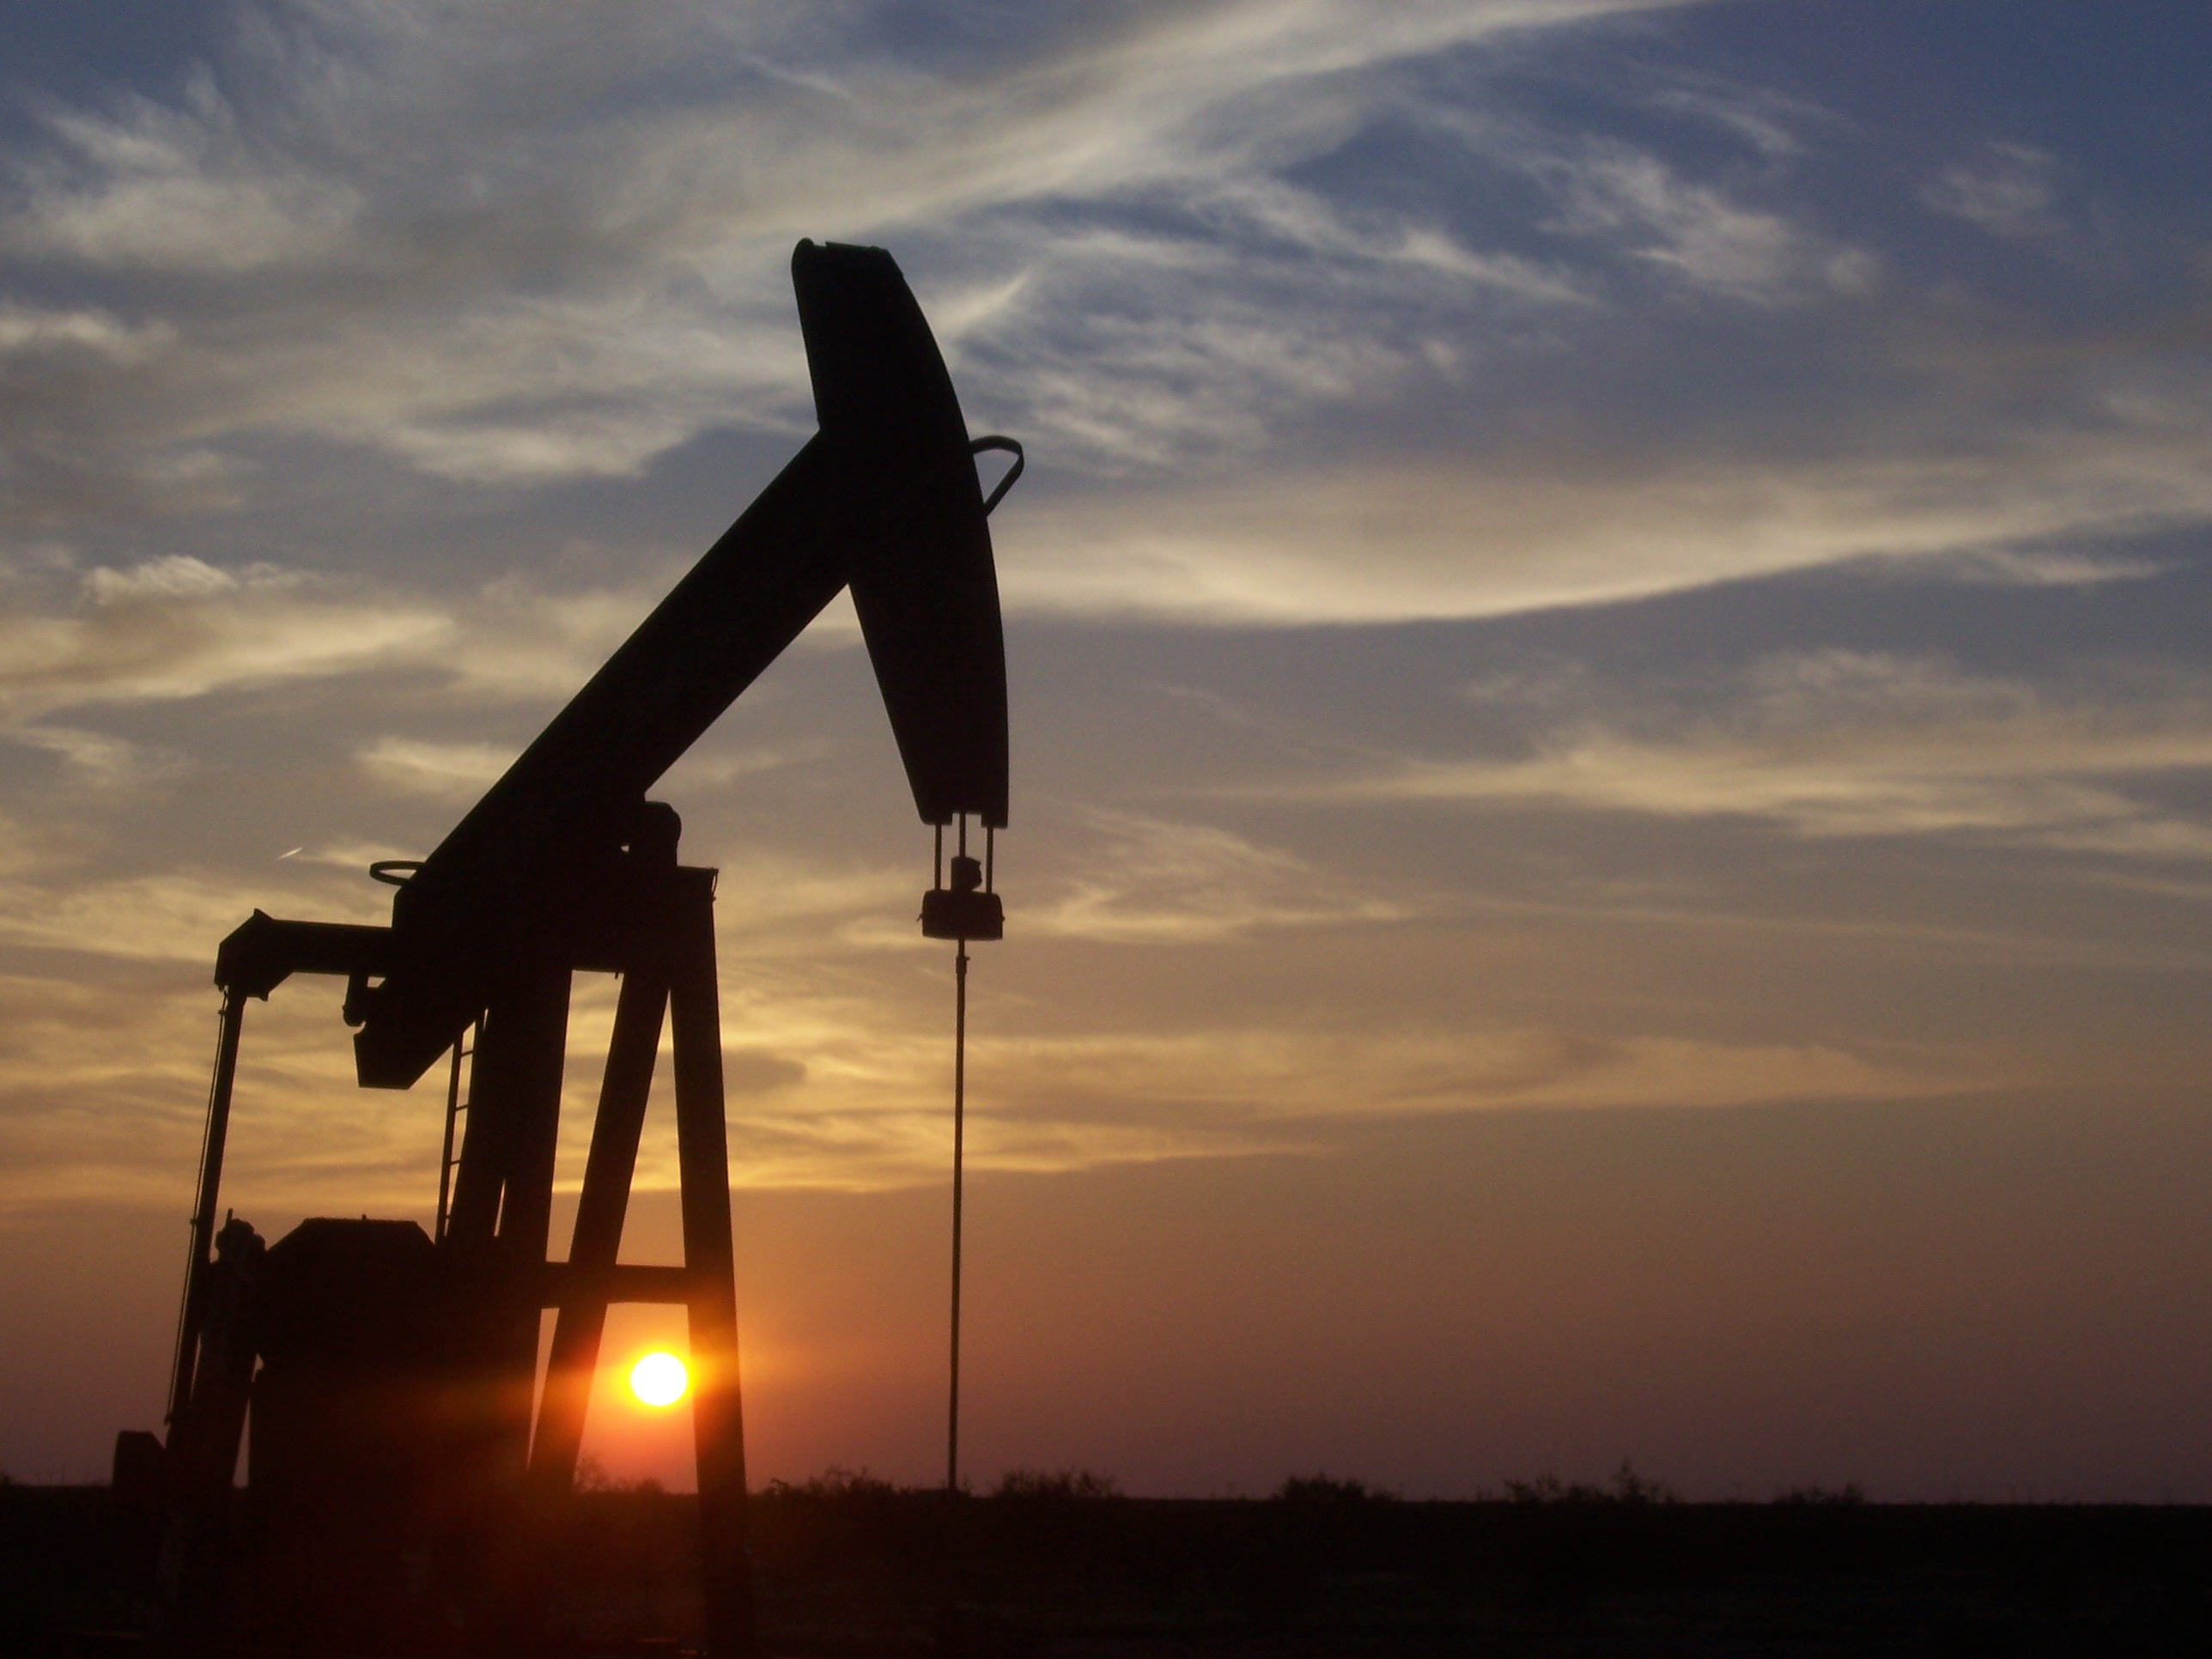
\includegraphics[width=0.4\linewidth]{West_Texas_Pumpjack}
	%\vspace{-10pt}
	\caption{Bomba de produção no oeste do Texas (fonte: wikimedia.org).}
	\label{fig:pump}
\end{figure}

O engenheiro de reservatórios tem conhecimento da sua proficiência em \textbf{R}, então enumerou as seguintes tarefas a executar.

\textbf{Nota:} Resolva as questões recorrendo, tanto quanto possível, a uma abordagem mais funcional e menos imperativa (i.e., usando funções e evitando usar ciclos, ou, dizendo de outro modo, tirando maior proveito das funcionalidades do \textbf{R}).

\begin{questions}
	\question Os dados estão disponíveis para download na seguinte localização: \url{http://tinyurl.com/welldata1}. Carregue os dados para uma estrutura de dados adequada.

	\begin{solution}
		\begin{rcode}
			# colocar entre aspas o caminho completo para o ficheiro
			welldata1 = read.csv("/home/julio/well_data1.dat")
		\end{rcode}
	\end{solution}
		
	\question Os dados recebidos contêm 7 variáveis:
	\begin{description}
		\item[X:] Coordenada X
		\item[Y:] Coordenada Y
		\item[Z:] Coordenada Z
		\item[facies:] diferentes tipos de rocha
		\item[density:] densidade da rocha
		\item[porosity:] porosidade da rocha
		\item[permeability:] permeabilidade da rocha (medida em mD)
	\end{description}
	Para evitar problemas na análise de dados, verifique se cada coluna ficou com o tipo de dados mais adequado, e ajuste conforme necessário.
	
	\begin{solution}
		É possível verificar o tipo de dados em cada coluna através da função \rinline{str}.
		\begin{rcode}
			> str(welldata1)
			'data.frame':	4438 obs. of  7 variables:
			$ X           : int  73 73 73 73 73 73 73 73 73 73 ...
			$ Y           : int  5 5 5 5 5 5 5 5 5 5 ...
			$ Z           : int  199 198 197 196 195 194 193 192 191 190 ...
			$ facies      : int  0 0 0 0 0 0 0 0 0 0 ...
			$ density     : num  2.39 2.4 2.4 2.42 2.42 ...
			$ porosity    : num  0.0549 0.0523 0.0522 0.0374 0.0361 0.039 0.0314 0.0464 0.0547 0.0537 ...
			$ permeability: num  6.81 4.38 5.78 3.51 2.54 ...
		\end{rcode}
		Verifica-se, assim, que todas as colunas são compostas por elementos numéricos. Ora, sendo a variável \textit{facies} categórica, o tipo de objecto mais apropriado é o \rinline{factor} e não o \rinline{numeric}. É, então, necessário alterar o tipo de elementos nesta coluna.
		
		\begin{rcode}
			> welldata1$facies = as.factor(welldata1$facies)
			> str(welldata1)
			'data.frame':	4438 obs. of  7 variables:
			$ X           : int  73 73 73 73 73 73 73 73 73 73 ...
			$ Y           : int  5 5 5 5 5 5 5 5 5 5 ...
			$ Z           : int  199 198 197 196 195 194 193 192 191 190 ...
			$ facies      : Factor w/ 4 levels "0","1","2","3": 1 1 1 1 1 1 1 1 1 1 ...
			$ density     : num  2.39 2.4 2.4 2.42 2.42 ...
			$ porosity    : num  0.0549 0.0523 0.0522 0.0374 0.0361 0.039 0.0314 0.0464 0.0547 0.0537 ...
			$ permeability: num  6.81 4.38 5.78 3.51 2.54 ...
		\end{rcode}
		
	\end{solution}
	
	\question As fácies correspondem a diferentes zonas no reservatório. Identifique quantas amostras recebeu de cada uma das zonas.
	
	\begin{solution}
		\begin{rcode}
			> table(welldata1$facies)
			
			0    1    2    3 
			2718  456  989  275 
		\end{rcode}
	\end{solution}
	
	\question Como primeira abordagem para identificar zonas de maior interesse (\textit{high pay zones}), obtenha um resumo com os estatísticos base de cada variável, em cada zona. Deste modo, poderá saber os valores típicos em cada uma das fácies.
	
	\begin{solution}
		Considerando que interessa apenas analizar os estatísticos base das variáveis relacionadas com as propriedades da rocha (últimas 3 colunas):
		\begin{rcode}
			by(welldata1[, 5:7], welldata1$facies, summary)
		\end{rcode}
	\end{solution}
	
	\question Outra estratégia consiste em encontrar as amostras com maiores valores de porosidade ($\geq 0,3$). Identifique essas amostras. Qual é a zona com maior número dessas amostras?
	
	\begin{solution}
		\begin{rcode}
			high.poro = subset(welldata1, welldata1$porosity >= 0.3)
			
			> table(high.poro$facies)
			
			0  1  2  3 
			0  0 59  0 
		\end{rcode}
	\end{solution}
	
	\question Entretanto, recebeu dados adicionais, que foram recolhidos mais tarde. Foram enviados através da ligação \url{http://tinyurl.com/welldata2}. Este novo conjunto de dados contém as seguintes variáveis:
	\begin{description}
		\item[X:] Coordenada X
		\item[Y:] Coordenada Y
		\item[Z:] Coordenada Z
		\item[Vp:] Velocidade das ondas P (km/s)
		\item[Vs:] Velocidade das ondas S (km/s)
	\end{description}
	Foi-lhe passada a informação de que o processo de aquisição de dados teve alguns problemas, e que é possível que tenha recebido a mesma amostra mais do que uma vez. Tome as medidas necessárias para corrigir esse possível erro.
	
	\begin{solution}
		\begin{rcode}
			# este ficheiro está separado por tabulações e não por vírgulas
			welldata2 = read.delim("/home/julio/well_data2.dat")
			# encontrar e remover registos em duplicado
			welldata2 = subset(welldata2, !duplicated(welldata2))
		\end{rcode}
	\end{solution}
	
	\question Com esse percalço ultrapassado, pode agora proceder à junção dos dois conjuntos de dados. Verifique as variáveis que têm em comum, e junte-os de acordo com as mesmas.
	\begin{solution}
		\begin{rcode}
			# verificar que variáveis têm em comum
			> intersect(names(welldata1), names(welldata2))
			[1] "X" "Y" "Z"
			# juntar
			welldata = merge(welldata1, welldata2)
			
		\end{rcode}
	\end{solution}
	
	\question Embora já tenha preparado todos os dados disponíveis, pode ainda ajudar na próxima etapa da modelação do reservatório, providenciado duas variáveis úteis. A impedância acústica é dada pelo produto da densidade com a velocidade sísmica, que varia entre diferentes camadas de rocha. Adicione duas colunas ao conjunto de dados:
	\begin{description}
		\item[Ip:] impedância acústica considerando as ondas P
		\item[Is:] impedância acústica considerando as ondas S
	\end{description}
	
	\begin{solution}
		\begin{rcode}
			welldata = transform(welldata, Ip = Vp * density, Is = Vs * density)
		\end{rcode}
	\end{solution}
	
	\question O seu trabalho está concluído. Agora, resta prepará-lo para ser entregue. Guarde os dados que preparou num formato de ficheiro apropriado.
	
	\begin{solution}
		\begin{rcode}
			write.csv(welldata, "/home/julio/welldata.dat", row.names=F)
		\end{rcode}
	\end{solution}

\end{questions}

\end{document}